\chapter{Bioethics: Designer Children}

These notes follow Michael Sandel's thirteenth \emph{Justice} lecture at CCCB, in the LazyLearn track curated by LazyingArt LLC with Video2Book. The lecture advances by a sequence of conceptual forks rather than by technical derivations: first a hard case about deafness, then a widening inquiry into the meaning of health, then a market analysis of reproductive choice, and finally a political question about who will set the limits of biotechnology. We can write the argumentative spine compactly, but we should keep the lecture's narrated rhythm on the page.

\section{The Opening Case: A Deaf Couple and a Deaf Child}

We begin, as Sandel begins, with a story rather than with a principle. A lesbian couple wanted a child, wanted the child to be born deaf, and because both partners were themselves deaf, they sought out a sperm donor who was also deaf and who came from a family with five generations of deafness. They conceived a child, and the child was born deaf. The point of the case is not statistical genetics. It is the moral meaning of intentional selection.

The opening broadcast graphic is sparse, but it captures the lecture's initial setup very well: a couple, a donor, and a child, arranged in that order from left to right.

\begin{figure}[h]
\centering

\includegraphics[width=0.62\textwidth]{lecture_13_figure_02.png}
\end{figure}

The screenshot does not contain labels, arrows, or written genetics. It gives us only a visible sequence,
\begin{equation}
\text{couple}
\qquad
\text{donor}
\qquad
\text{child},
\end{equation}
together with repeated head-adjacent markers on the adults and the infant. In context the lecture's meaning is clear enough: the couple seeks a child who shares the trait they themselves have. But the image itself remains intentionally schematic, and it is useful to keep that schematic character in our notes.

A cleaned redraw, preserving only the visible arrangement, is therefore enough:

\begin{figure}[h]
\centering
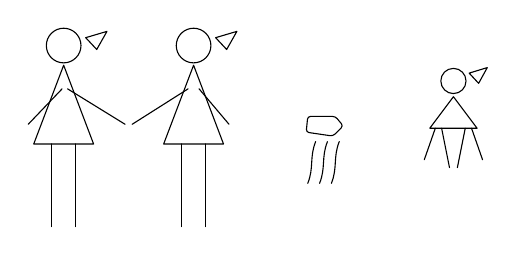
\begin{tikzpicture}[x=1cm,y=1cm,line cap=round,line join=round]
\draw (0,3.0) circle (0.22);
\draw (0,2.75)--(-0.38,1.75)--(0.38,1.75)--cycle;
\draw (-0.15,1.75)--(-0.15,0.7);
\draw (0.15,1.75)--(0.15,0.7);
\draw (-0.02,2.45)--(-0.45,2.0);
\draw (0.05,2.45)--(0.78,2.0);
\draw (0.28,3.10)--(0.55,3.18)--(0.42,2.95)--cycle;

\draw (1.65,3.0) circle (0.22);
\draw (1.65,2.75)--(1.27,1.75)--(2.03,1.75)--cycle;
\draw (1.50,1.75)--(1.50,0.7);
\draw (1.80,1.75)--(1.80,0.7);
\draw (1.58,2.45)--(0.87,2.0);
\draw (1.72,2.45)--(2.10,2.0);
\draw (1.93,3.10)--(2.20,3.18)--(2.07,2.95)--cycle;

\draw[rounded corners=1pt] (3.10,2.10)--(3.45,2.10)--(3.55,1.98)--(3.42,1.85)--(3.08,1.90)--cycle;
\draw (3.20,1.78) .. controls (3.12,1.58) and (3.18,1.45) .. (3.10,1.25);
\draw (3.35,1.78) .. controls (3.27,1.58) and (3.33,1.45) .. (3.25,1.25);
\draw (3.50,1.78) .. controls (3.42,1.58) and (3.48,1.45) .. (3.40,1.25);

\draw (4.95,2.55) circle (0.16);
\draw (4.95,2.35)--(4.65,1.95)--(5.25,1.95)--cycle;
\draw (4.72,1.95)--(4.58,1.55);
\draw (5.18,1.95)--(5.32,1.55);
\draw (4.80,1.95)--(4.90,1.45);
\draw (5.10,1.95)--(5.00,1.45);
\draw (5.15,2.65)--(5.38,2.72)--(5.27,2.52)--cycle;
\end{tikzpicture}
\end{figure}

Now the philosophical pressure enters. Sandel reports the couple's own defense: deafness, they argue, is not a disability but a distinctive identity. That turns the case at once into a fork:
\begin{equation}
\text{deafness}
\stackrel{?}{=}
\text{disability}
\qquad \text{or} \qquad
\text{deafness}
\stackrel{?}{=}
\text{distinctive identity}.
\end{equation}

\subsection{Question \& Answer}

\paragraph{Question.} Is deafness here being treated as a disability imposed on the child, or as a distinctive identity intentionally shared?

\paragraph{Answer.} Sandel does not settle the issue by fiat. The immediate lesson of the case is methodological rather than conclusory: this is precisely the kind of borderline case that forces us to ask what counts as health, what counts as harm, and what kind of human difference medicine may permissibly aim to produce or prevent.

\section{Borderline Cases and the Meaning of Health}

From the deaf-child case Sandel does not move directly to a verdict. He widens the inquiry. If deafness can be described either as pathology or as identity, then what are we to say about a tendency to obesity, or baldness, or the straightening of teeth in orthodontia? At this point the lecture ceases to be about one controversial story and becomes an inquiry into a general classificatory problem.

The problem is compactly expressed as
\begin{equation}
\text{intervention}
\stackrel{?}{=}
\text{medically necessary}
\qquad \text{or} \qquad
\text{purely preferential}.
\end{equation}
That is the first genuinely formal move of the lecture. Once we place the examples side by side, we can no longer rely on an unexamined distinction between cure and choice. We have to decide what counts as health in the first place.

\paragraph{Worked inference.} Sandel's argument in this stretch can be written as a short implication chain:
\begin{align}
\text{borderline cases}
&\Longrightarrow
\text{contested meaning of health},\\
\text{contested meaning of health}
&\Longrightarrow
\text{need for public debate about technological limits}.
\end{align}
And Sandel states the endpoint explicitly:
\begin{align}
\text{new genetic technology}
&\Longrightarrow
\text{public debate about the meaning of health},\\
\text{public debate about health}
&\Longrightarrow
\text{public debate about the limits of genetic technology}.
\end{align}

\subsection{Question \& Answer}

\paragraph{Question.} When is an intervention medically necessary, and when is it merely preferential?

\paragraph{Answer.} The lecture's answer is that no fixed technical formula is available in advance. The distinction must itself be argued about. Once biotechnology enables us to alter traits at the boundary between pathology and variation, public life must decide what it means to call something a disease, an impairment, an identity, or a preference.

\section{Popular Culture and the Logic of Selection}

Only after establishing the boundary problem does Sandel make a surprising turn. Some of the deepest worries about biotechnology, he says, have come to us through popular culture, through novels and film. The point of the move is not literary ornament. It is to make visible a logic that might otherwise seem abstract.

The filmic sequence he invokes is garbled in transcript detail, but its function is clear enough. A set of possible children is screened, compared, and selected. The choice is no longer simply whether to have a child, but which child to have. In compact form, the imagined logic is
\begin{equation}
\text{screening} + \text{parental preference}
\Longrightarrow
\text{selection among possible children}.
\end{equation}
That transition matters because it shifts the horizon of the lecture. We are no longer asking only whether biotechnology can heal. We are asking what happens when biotechnology becomes a medium of selection.

The lecture therefore moves from border cases in health to a broader concern about mastery. Before Sandel names that concern directly, however, he turns back from fiction to a real market institution.

\section{Cryobank, Catalogs, and the Market for Traits}

Sandel's next example is California Cryobank, a successful for-profit sperm bank. This is the lecture's first institutional case of biotechnology operating in overtly commercial form. Sperm is sold, donors are screened, very few are accepted, and donor characteristics are cataloged in detail. Sandel's pacing matters here. He first lays out the mechanics of the market; only then does he draw the moral conclusion.

\paragraph{Worked market example.} The structure of the example can be written as
\begin{align}
\text{cataloged donor traits}
&=
\text{physical characteristics}
+
\text{ethnic origin}
+
\text{college major}
+\cdots,\\
\text{compensation}
&\leq
\$900 \text{ per month},\\
\text{cataloged donor traits}
+
\text{consumer choice}
&\Longrightarrow
\text{reproductive selection as market behavior}.
\end{align}
The numerical datum is small compared to the philosophical claim, but it is important. Once a price appears, the transaction takes on a recognizably commercial form. The slogan ``Ivy League sperm'' sharpens the point even further: the market is not merely facilitating reproduction, it is advertising ranked human traits.

\subsection{Question \& Answer}

\paragraph{Question.} When does reproductive choice become consumer selection?

\paragraph{Answer.} For Sandel, the shift occurs once reproductive materials are screened, ranked, cataloged, and priced according to desirable traits. At that point the grammar of the transaction changes. What had looked like assistance in childbearing begins to look like customization within a market.

Sandel then draws a crucial distinction. The company, he says, has no explicit eugenic purpose. It simply wants to make money. This matters because the danger he is isolating is not confined to grand ideological programs. Ordinary commercial logic is enough to begin transforming children and childbearing into extensions of consumer society.

\section{Designer Babies and the Expansion of Parental Responsibility}

The lecture now widens again. Cryobank is not the end of the argument, but a precursor to a larger prospect: designer babies. A fertility clinic, Sandel notes, proposes to let parents choose traits such as sex, hair color, eye color, and skin color. The point is no longer donor selection alone. The point is the growing power to redesign the child as an object of choice.

Here the lecture's next formal move is especially important:
\begin{equation}
\text{genetic design of children}
\Longrightarrow
\text{explosion of parental responsibility}.
\end{equation}
Why an explosion? Because once traits can be selected, they no longer appear simply as gifts, accidents, or inheritances. They become attributable to decision. Sandel therefore adds a second implication:
\begin{equation}
\text{expanded design responsibility}
\Longrightarrow
\text{damage to the parent-child relation}.
\end{equation}
He makes the point concretely. Children might come to hold parents responsible for their height, their physical appearance, perhaps even their academic performance. This is a striking inversion. A technology introduced in the name of greater parental choice can end by burdening parenthood with a new and corrosive form of accountability.

\subsection{Question \& Answer}

\paragraph{Question.} Would genetic design deepen parental agency, or corrupt the parent-child relation?

\paragraph{Answer.} Sandel's answer is that the increase in agency comes at the cost of the relation itself. The more traits are chosen, the less the child is received as given and the more the child is treated as the result of a project. That change in stance threatens to replace acceptance with manufacture, and care with design responsibility.

\section{Commodification and Moral Judgment}

By now the lecture is ready for its strongest moral claim. Sandel says that what is dangerous about these consumer uses of biotechnology is not merely that they are novel or powerful. It is that they alter the moral meaning of children and childbearing. The argument can be compressed into one line:
\begin{equation}
\text{children and childbearing}
\Longrightarrow
\text{extension of consumer society}
\Longrightarrow
\text{commodification of children}.
\end{equation}
This is not for Sandel a merely sociological observation. It is a moral diagnosis. Once childbearing becomes an occasion for preference-satisfaction in a market setting, children come to resemble consumer goods rather than beings to be welcomed and educated.

The lecture therefore arrives at its explicit normative conclusion:
\begin{equation}
\text{consumer uses of genetic engineering}
\Longrightarrow
\text{morally impermissible}.
\end{equation}
Notice the order. Sandel does not begin with this sentence. He earns it through the opening case, the widening list of border cases, the filmic illustration, the commercial example, and the analysis of parental responsibility. The moral verdict is the payoff of that sequence.

\section{Market or Democracy: Who Decides the Limits?}

The lecture closes by turning from moral diagnosis to institutional choice. Once the danger has been named, the question is not merely whether it exists, but who will decide how to respond to it. Sandel's closing fork is almost theorem-like:
\begin{equation}
\text{ultimate decision agency}
=
\text{market}
\;\;\text{or}\;\;
\text{democratic institutions}.
\end{equation}
And the sharper conditional is the one on which the lecture ends:
\begin{equation}
\text{no public collective decision}
\Longrightarrow
\text{market decides by default}.
\end{equation}
This final step is essential. The lecture is not satisfied with private moral disapproval. If democratic societies do not publicly deliberate about the ethical limits of biotechnology, then those limits will not remain undecided in practice. They will be set by the logic of demand, supply, and competitive advantage.

\subsection{Question \& Answer}

\paragraph{Question.} If society does not decide collectively, who decides by default?

\paragraph{Answer.} The market. That is Sandel's closing institutional point. The alternative is not decision versus no decision. It is democratic decision versus market rule. The lecture ends, accordingly, not with resignation but with the hope for a public debate and a public determination of biotechnology's ethical limits.

\section{Summary}

Sandel's lecture moves from a hard case to a general problem, from a general problem to market institutions, and from market institutions to political responsibility. The deaf-child case forces the opening fork between disability and identity. The list of obesity, baldness, and orthodontia widens that fork into a broader debate about the meaning of health. The Cryobank example and the prospect of designer babies then show how reproductive choice can become consumer selection, how parental responsibility can expand into design responsibility, and how children can come to be treated as commodities.

The final claim is both moral and political. Consumer uses of genetic engineering are, for Sandel, morally impermissible not only because they invite risky choices, but because they threaten to transform the relation between parents and children. And if democratic societies do not decide collectively where the limits of biotechnology lie, the market will decide for them.